\chapter{Prediksi dengan Random Forest}

\section{Lusia Violita Aprilian/1164080}
\subsection{Teori}
\begin{enumerate}
\item Random Forest
	\begin{itemize}
	\item Random Forest diperkenalkan dan diselidiki untuk memprediksi aktivitas biologis kategoris atau kategoris suatu senyawa berdasarkan pada deskripsi kuantitatif dari struktur molekul senyawa. Random Forest adalah ensemble dari pohon klasifikasi atau regresi yang tidak ditandai yang dibuat dengan menggunakan sampel bootstrap dari data pelatihan dan pemilihan fitur acak dalam induksi pohon. Prediksi dibuat dengan menggabungkan (suara terbanyak atau rata-rata) prediksi ensemble.
	\item Gambar Random Forest
		\begin{figure}[!hbtp]
		\centering
		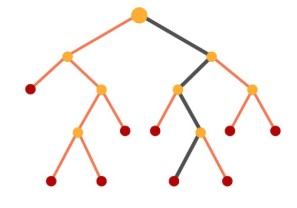
\includegraphics[scale=0.5]{figures/j1.jpg}
		\caption{Random Forest}
		\label{contoh}
		\end{figure}
	\end{itemize}

\item Membaca Dataset
	\begin{itemize}
	\item Berikut adalah cara membaca dataset :
		\begin{enumerate}
			\item Buka Anaconda Navigator lalu jalankan Spyder, kemudian import libraries yang dibutuhkan.
			\item Masukkan kode python untuk membaca file csv, lalu jalankan.
				\begin{figure}[!hbtp]
				\centering
				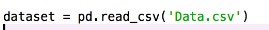
\includegraphics[scale=0.8]{figures/j41.jpg}
				\caption{Kode Python}
				\label{contoh}
				\end{figure}
			\item Maka pada window console akan menampilkan pesan berikut :
				\begin{figure}[!hbtp]
				\centering
				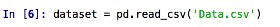
\includegraphics[scale=0.9]{figures/j42.jpg}
				\caption{Pesan Window Console}
				\label{contoh}
				\end{figure}
			\item Dari explorer dapat terlihat dataset yang terimport.
				\begin{figure}[!hbtp]
				\centering
				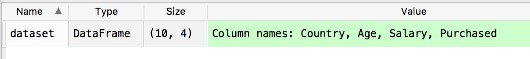
\includegraphics[scale=0.6]{figures/j43.jpg}
				\caption{Dataset}
				\label{contoh}
				\end{figure}
			\item Lalu klik dataset cell, maka akan muncul seperti berikut :
				\begin{figure}[!hbtp]
				\centering
				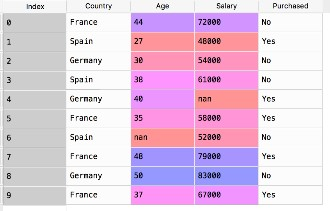
\includegraphics[scale=0.7]{figures/j44.jpg}
				\caption{Hasil Dataset Cell}
				\label{contoh}
				\end{figure}
			\item Seperti yang terlihat pada gambar tersebut dataset ini memiliki Kolom Country, Age, dan Salary sebagai independent variable-nya dan kolom Purchased sebagai dependent variable-nya.
			\item Selanjutnya buat 2 matrix of features yang berisi values dari independent variable dan dependent variable.
			\item Lalu tuliskan perintah berikut :
				\begin{figure}[!hbtp]
				\centering
				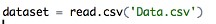
\includegraphics[scale=0.9]{figures/j45.jpg}
				\caption{Perintah}
				\label{contoh}
				\end{figure}
			\item Perintah yang telah dibuat di atas akan membuat sebuah global environment baru dan muncul dataset.
			\item Klikdataset tersebut maka muncul tabel berisi dataset.
		\end{enumerate}
	\end{itemize}

\item Cross Validation
	\begin{itemize}
		\item Cross validation adalah metode statistik yang digunakan untuk memperkirakan keterampilan model pembelajaran mesin. Ini biasanya digunakan dalam pembelajaran mesin yang diterapkan untuk membandingkan dan memilih model untuk masalah pemodelan prediktif yang diberikan karena mudah dipahami, mudah diimplementasikan, dan menghasilkan estimasi keterampilan yang umumnya memiliki bias lebih rendah daripada metode lainnya.
	\end{itemize}
	
\item Menjelaskan Arti Score
	\begin{itemize}
		\item Maksud arti score 44\% pada random forest adalah hasil akurasi.
		\item Maksud arti score 27\% pada decission tree adalah presentasi hasil dari perhitungan dataset.
		\item Maksud arti score 29\% dari SVM adalah hasil pendekatan neural network.
		\item Hasil tersebut didapat dari hasil valdasi silang untuk memastikan bahwa membagi  training test dengan cara yang berbeda. Sehingga didapat outputnya 44\% untuk hutan acak, 27\% untuk pohon keputusan, dan 29\% untuk SVM.
	\end{itemize}

\item Cara Membaca Confusion Matriks
	\begin{itemize}
		\item Mari kita lihat contoh klasifikasi biner berikut ini, yang menunjukkan berapa kali model telah membuat prediksi objek yang benar:
			\begin{figure}[!hbtp]
			\centering
			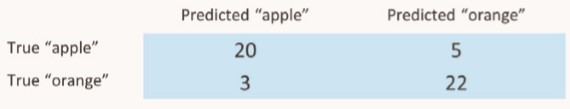
\includegraphics[scale=0.5]{figures/j2a.jpg}
			\caption{Tabel Confusion Matriks}
			\label{contoh}
			\end{figure}
		\item Dalam tabel tersebut, baris apple dan orange mengacu pada kasus di mana objek tersebut sebenarnya sebuah apel atau sebuah jeruk. Kolom merujuk pada prediksi yang dibuat oleh model. Kita melihat bahwa dalam contoh ada 20 apel yang diprediksi dengan benar, sementara ada 5 apel yang salah diidentifikasi sebagai jeruk. Idealnya, confusion matriks harus memiliki semua nilai nol, kecuali untuk diagonal. Di sini kita dapat menghitung akurasi dengan menambahkan angka secara diagonal, sehingga ini semua adalah contoh yang diklasifikasikan dengan benar, dan membagi jumlah tersebut dengan jumlah semua angka dalam matriks:
			\begin{figure}[!hbtp]
			\centering
			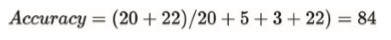
\includegraphics[scale=0.5]{figures/j2b.jpg}
			\caption{Rumus Confusion Matriks}
			\label{contoh}
			\end{figure}
		\item Sehingga dari perhitungan tersebut kita mendapat akurasi 84%.
		\item Berikut adalah gambar klasifikasi biner :
			\begin{figure}[!hbtp]
			\centering
			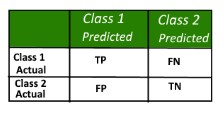
\includegraphics[scale=0.5]{figures/j2c.jpg}
			\caption{Confusion Matriks}
			\label{contoh}
			\end{figure}
	\end{itemize}
	
\item Voting Pada Random Forest
	\begin{itemize}
		\item Voting pada random forest merupakan metode yang paling umum digunakan setelah classifier membuat keputusan.
		\item Gambar voting pada random forest
			\begin{figure}[!hbtp]
			\centering
			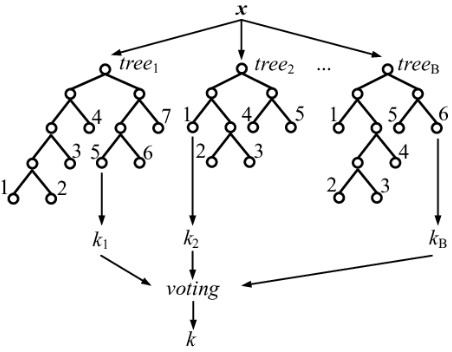
\includegraphics[scale=0.5]{figures/j3.jpg}
			\caption{Voting Pada Random Forest}
			\label{contoh}
			\end{figure}
	\end{itemize}

\end{enumerate}

\subsection{Praktek}
\begin{enumerate}
\item Aplikasi Sederhana Menggunakan Pandas
	\begin{figure}[!hbtp]
	\centering
	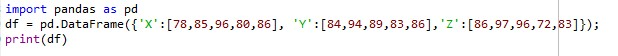
\includegraphics[scale=0.5]{figures/k1a.jpg}
	\caption{Aplikasi Pandas}
	\label{contoh}
	\end{figure}
	\par Penjelasan kodingan :
		\begin{enumerate}
		\item Memanggil library.
		\item Membuat variable dengan data frame.
		\item Menampilkan hasil
		\end{enumerate}
	\par Sehingga menghasilkan :
	\begin{figure}[!hbtp]
	\centering
	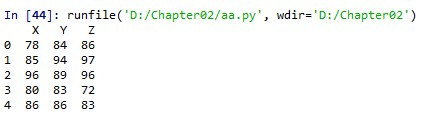
\includegraphics[scale=0.5]{figures/k1b.jpg}
	\caption{Hasil Pandas}
	\label{contoh}
	\end{figure}
\item Aplikasi Sederhana Menggunakan Numpy
	\begin{figure}[!hbtp]
	\centering
	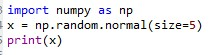
\includegraphics[scale=0.5]{figures/k2a.jpg}
	\caption{Aplikasi Numpy}
	\label{contoh}
	\end{figure}
	\par Penjelasan kodingan :
		\begin{enumerate}
		\item Memanggil library
		\item Membuat variable dengan value random dan size 5
		\item Menampilkan hasil value
		\end{enumerate}
	\par Sehingga menghasilkan :
	\begin{figure}[!hbtp]
	\centering
	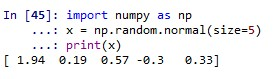
\includegraphics[scale=0.5]{figures/k2b.jpg}
	\caption{Hasil Numpy}
	\label{contoh}
	\end{figure}
\item Aplikasi Sederhana Menggunakan Matplotlib
	\begin{figure}[!hbtp]
	\centering
	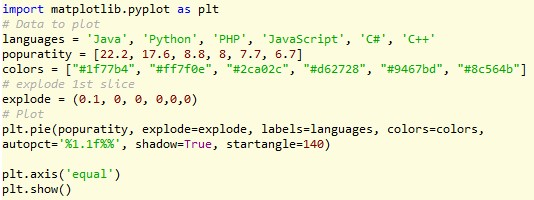
\includegraphics[scale=0.5]{figures/k3a.jpg}
	\caption{Aplikasi Matplotlib}
	\label{contoh}
	\end{figure}
	\par Penjelasan kodingan :
		\begin{enumerate}
		\item Memanggil library
		\item Membuat variable yang berisi bahasa pemrograman
		\item Membuat variable yang berisi popularitas
		\item Membuat variable untuk menentukan warna
		\item Membuat variable untuk explode
		\item Membuat diagram pie atau yang berbentuk lingkaran
		\item Membuat garis koordinat
		\item Menampilkan hasil
		\end{enumerate}
	\par Sehingga menghasilkan :
	\begin{figure}[!hbtp]
	\centering
	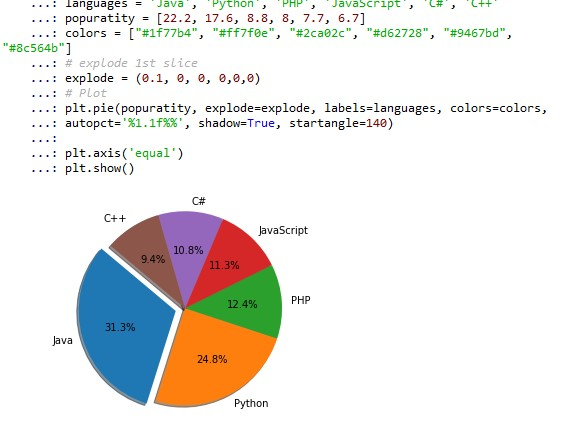
\includegraphics[scale=0.5]{figures/k3b.jpg}
	\caption{Hasil Matplotlib}
	\label{contoh}
	\end{figure}
\item Program Klasifikasi Random Fores
	\begin{itemize}
		\item Yang pertama dataset akan dibaca.
			\begin{figure}[!hbtp]
			\centering
			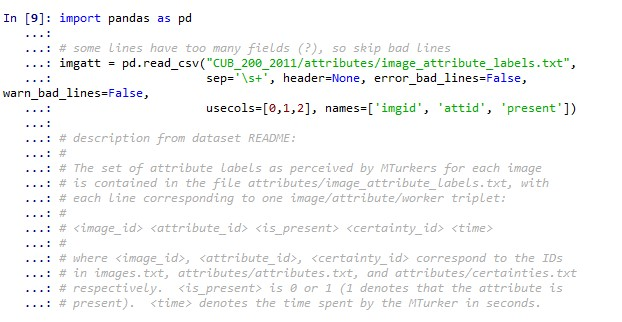
\includegraphics[scale=0.5]{figures/k41.jpg}
			\caption{Membaca Data File}
			\label{contoh}
			\end{figure}
		 \item Selanjutnya sebagian data awal akan dilihat dengan menggunkan listing.
		 	\begin{figure}[!hbtp]
			\centering
			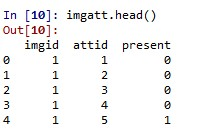
\includegraphics[scale=0.5]{figures/k42.jpg}
			\caption{Melihat Data Sebagian}
			\label{contoh}
			\end{figure}
		\item Selanjutnya jumlah data dilihat dengan menggunakan listing.
			\begin{figure}[!hbtp]
			\centering
			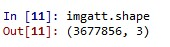
\includegraphics[scale=0.5]{figures/k43.jpg}
			\caption{Melihat Jumlah Data}
			\label{contoh}
			\end{figure}
		\item Lalu atribut diubah menjadi kolom dengan menggunakan perintah pivot.
			\begin{figure}[!hbtp]
			\centering
			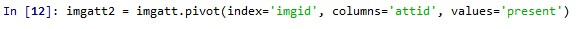
\includegraphics[scale=0.5]{figures/k44.jpg}
			\caption{Mengubah menjadi kolom}
			\label{contoh}
			\end{figure}
		\item Selanjutnya atribut yang telah diubah, sebagian data awalnya akan dilihat dengan menggunkan listing kembali.
			\begin{figure}[!hbtp]
			\centering
			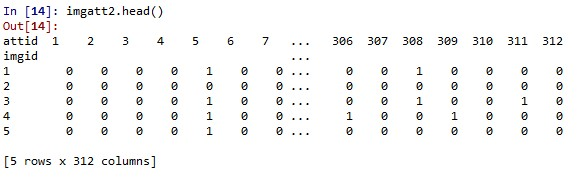
\includegraphics[scale=0.5]{figures/k45.jpg}
			\caption{Lihat sebagian data awal}
			\label{contoh}
			\end{figure}
		\item Selanjutnya atribut yang telah diubah, jumlah data dilihat dengan menggunakan listing kembali.
			\begin{figure}[!hbtp]
			\centering
			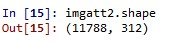
\includegraphics[scale=0.5]{figures/k46.jpg}
			\caption{Melihat jumlah data}
			\label{contoh}
			\end{figure}
		\item Lalu mengelompokkan burung kedalam spesies yang sama dengan dua kolom imgid dan label.
			\begin{figure}[!hbtp]
			\centering
			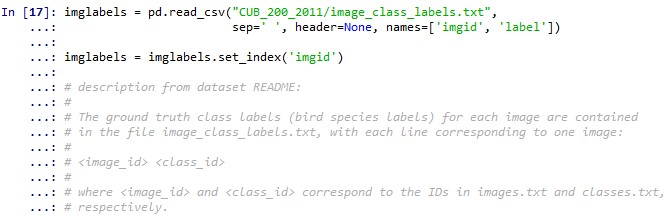
\includegraphics[scale=0.5]{figures/k47.jpg}
			\caption{Mengelompokkan burung}
			\label{contoh}
			\end{figure}
		\item Lalu melakukan pivot dimana imgid menjadi index.
			\begin{figure}[!hbtp]
			\centering
			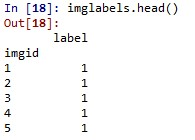
\includegraphics[scale=0.5]{figures/k48.jpg}
			\caption{Melalukan pivot}
			\label{contoh}
			\end{figure}
		\item Selanjutnya imgid, sebagian data awalnya akan dilihat dengan menggunkan listing untuk mengecek data.
			\begin{figure}[!hbtp]
			\centering
			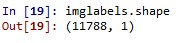
\includegraphics[scale=0.5]{figures/k49.jpg}
			\caption{Melihat data awal imgid}
			\label{contoh}
			\end{figure}
		\item Selanjutnya imgid, jumlah data dilihat dengan menggunakan listing untuk mengecek data.
			\begin{figure}[!hbtp]
			\centering
			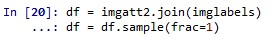
\includegraphics[scale=0.5]{figures/k410.jpg}
			\caption{Melihat jumlah data imgid}
			\label{contoh}
			\end{figure}
		\item Lalu melakukan join karena isi datanya adalah sama di antara dua data. Sehingga mendapatkan data ciri labelnya sehingga bisa dikategorikan.
			\begin{figure}[!hbtp]
			\centering
			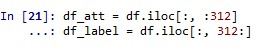
\includegraphics[scale=0.5]{figures/k411.jpg}
			\caption{Data ciri label dari join}
			\label{contoh}
			\end{figure}
		\item Kemudian label yang didepan di drop dan berikan label pada data yang telah dilakukan join dengan perintah listing.
			\begin{figure}[!hbtp]
			\centering
			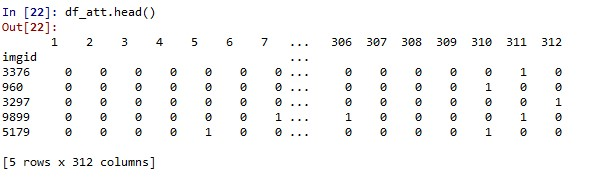
\includegraphics[scale=0.5]{figures/k412.jpg}
			\caption{Mengubah menjadi kolom}
			\label{contoh}
			\end{figure}
		\item Lalu cek kembali isinya dengan perintah listing. 
			\begin{figure}[!hbtp]
			\centering
			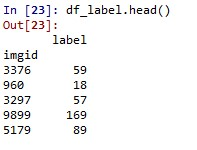
\includegraphics[scale=0.5]{figures/k413.jpg}
			\caption{Melihat isi data frame}
			\label{contoh}
			\end{figure}
		\item Kemudian data dibagi menjadi dua bagian, dimana 8000 row pertama merupakan data training dan sisanya adalah data testing.
			\begin{figure}[!hbtp]
			\centering
			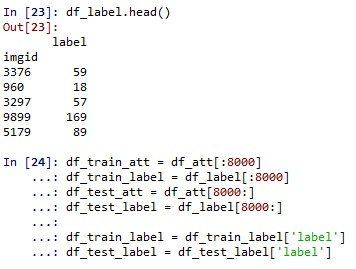
\includegraphics[scale=0.5]{figures/k414.jpg}
			\caption{Membagi data}
			\label{contoh}
			\end{figure}
		\item Kelas random forest selanjuknya dipanggil dengan RandomForestClassifier, dengan banyak kolom yang telah ditentukan oleh max feature.
			\begin{figure}[!hbtp]
			\centering
			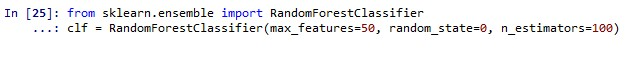
\includegraphics[scale=0.5]{figures/k415.jpg}
			\caption{Kelas Random Forest}
			\label{contoh}
			\end{figure}
		\item Kemudian untuk membangun random forest dilakukan perintah fitting dengan maksimum fitur sebanyak 50.
			\begin{figure}[!hbtp]
			\centering
			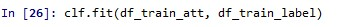
\includegraphics[scale=0.5]{figures/k416.jpg}
			\caption{Membangun Random forest}
			\label{contoh}
			\end{figure}
		\item Kemudian lihat hasilnya dengan perintah predict.
			\begin{figure}[!hbtp]
			\centering
			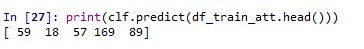
\includegraphics[scale=0.5]{figures/k417.jpg}
			\caption{Melihat hasil}
			\label{contoh}
			\end{figure}
		\item Lalu akan terlihat hasil score dari klasifikasi.
			\begin{figure}[!hbtp]
			\centering
			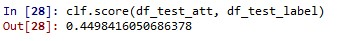
\includegraphics[scale=0.5]{figures/k418.jpg}
			\caption{Lihat hasil score}
			\label{contoh}
			\end{figure}
	\end{itemize}
\item Program Klasifikasi Confusion Matrix
	\begin{itemize}
		\item Setelah melakukan random forest kemudian dipetakan ke dalam confusion matrix.
			\begin{figure}[!hbtp]
			\centering
			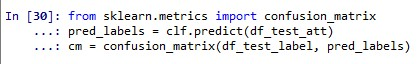
\includegraphics[scale=0.5]{figures/k51.jpg}
			\caption{Memetakan ke confusion matrix}
			\label{contoh}
			\end{figure}
		\item Lalu melihat hasilnya.
			\begin{figure}[!hbtp]
			\centering
			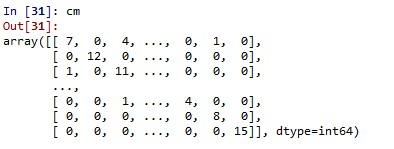
\includegraphics[scale=0.5]{figures/k52.jpg}
			\caption{Melihat hasil}
			\label{contoh}
			\end{figure}
		\item Kemudian dilakukan perintah plot.
			\begin{figure}[!hbtp]
			\centering
			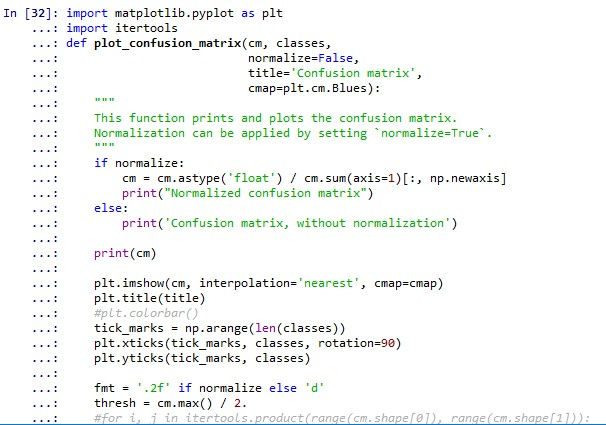
\includegraphics[scale=0.5]{figures/k53.jpg}
			\caption{Melakukan Plot}
			\label{contoh}
			\end{figure}
		\item Selanjutnya nama data akan di set agar plot sumbunya sesuai.
			\begin{figure}[!hbtp]
			\centering
			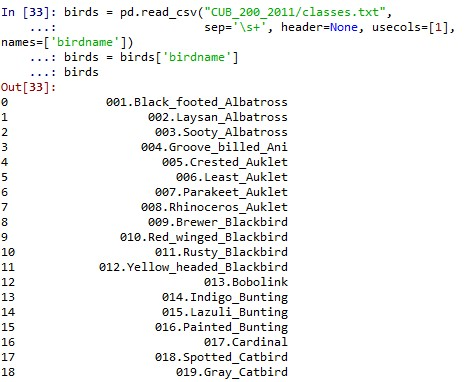
\includegraphics[scale=0.5]{figures/k54.jpg}
			\caption{Plotting nama data}
			\label{contoh}
			\end{figure}
		\item Setelah label berubah, maka dilakukan perintah plot.
		\begin{figure}[!hbtp]
			\centering
			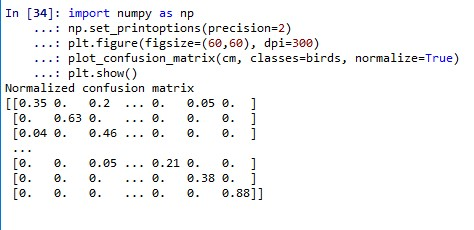
\includegraphics[scale=0.5]{figures/k55.jpg}
			\caption{Melakukan perintah plot}
			\label{contoh}
			\end{figure}
	\end{itemize}
\item Program Klasifikasi SVM dan Decision Tree
	\begin{enumerate}
		\item Program Decision Tree
			\par Mengklasifikasikan dataset yang sama menggunakan decision tree.
				\begin{figure}[!hbtp]
				\centering
				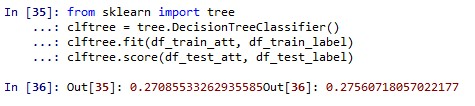
\includegraphics[scale=0.5]{figures/k61.jpg}
				\caption{Klasifkasi menggunakan decision tree}
				\label{contoh}
				\end{figure}
		\item Program Klasifikasi SVM
			\par Mengklasifikasikan dataset yang sama menggunakan SVM.
				\begin{figure}[!hbtp]
				\centering
				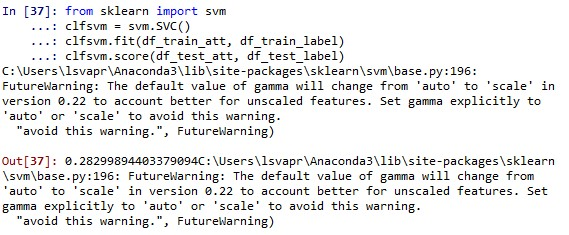
\includegraphics[scale=0.5]{figures/k62.jpg}
				\caption{Klasifikasi menggunakan SVM}
				\label{contoh}
				\end{figure}
	\end{enumerate}
\item Program Cross Validation
	\begin{itemize}
		\item Melakukan pengecekan cross validation untuk random forest.
			\begin{figure}[!hbtp]
			\centering
			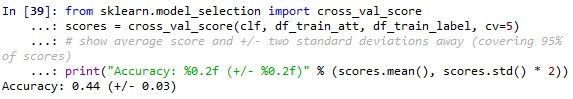
\includegraphics[scale=0.5]{figures/k71.jpg}
			\caption{Pengecekan cross validation random forest}
			\label{contoh}
			\end{figure}
		\item Melakukan pengecekan cross validation untuk decission tree.
			\begin{figure}[!hbtp]
			\centering
			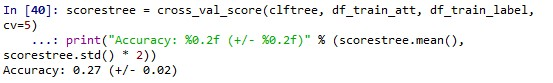
\includegraphics[scale=0.5]{figures/k72.jpg}
			\caption{Pengecekan cross validation decision tree}
			\label{contoh}
			\end{figure}
		\item Melakukan pengecekan cross validation untuk SVM.
			\begin{figure}[!hbtp]
			\centering
			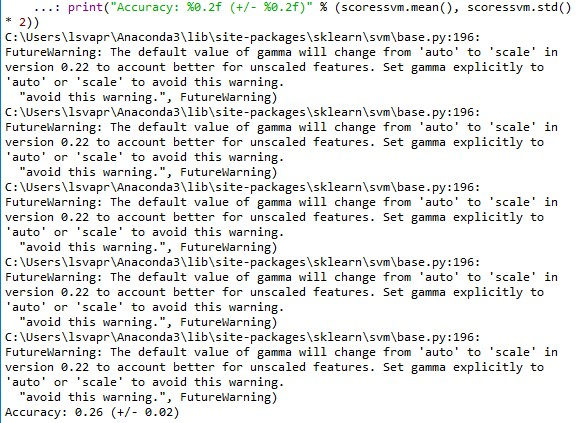
\includegraphics[scale=0.5]{figures/k73.jpg}
			\caption{Pengecekan cross validation SVM}
			\label{contoh}
			\end{figure}
	\end{itemize}
\item Program Pengamatan Komponen Informasi
	\begin{itemize}
		\item Melakukan pengamatan komponen informasi untuk menetahui berapa banyak tree yang dibuat, atribut yang dipakai, dan informasi lainnya.
			\begin{figure}[!hbtp]
			\centering
			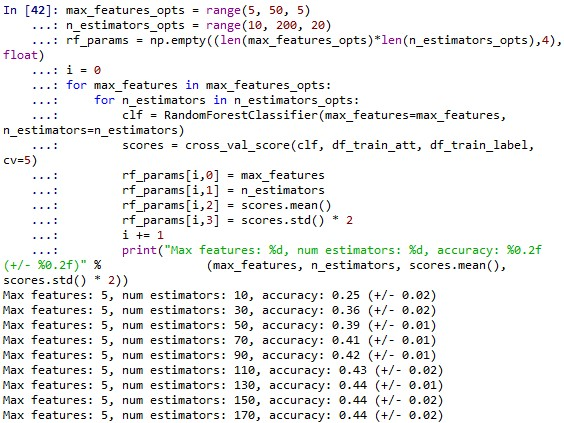
\includegraphics[scale=0.5]{figures/k81.jpg}
			\caption{Pengamatan Komponen}
			\label{contoh}
			\end{figure}
		\item Melakukan plot informasi agar bisa dibaca.
			\begin{figure}[!hbtp]
			\centering
			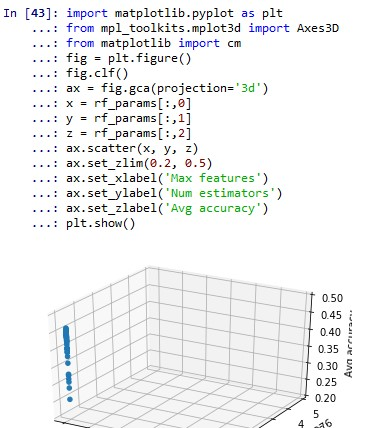
\includegraphics[scale=0.5]{figures/k82.jpg}
			\caption{Plot informasi}
			\label{contoh}
			\end{figure}
	\end{itemize}
\end{enumerate}

\subsection{Penanganan Error}
\begin{enumerate}
\item Skrinsut Error
	\begin{figure}[!hbtp]
	\centering
	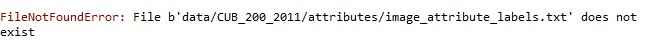
\includegraphics[scale=0.5]{figures/l1.jpg}
	\caption{Skrinsut Error}
	\label{contoh}
	\end{figure}
\item Tuliskan kode eror dan jenis errornya
	\par Kode Error = FileNotFoundError: File b'data/CUB 200 2011/attributes/image attribute labels . txt' does not exist
	\par Jenis Error = File not found
\item Solusi Pemecahan Masalah Error
\par Solusi dari error yang terjadi pada nomor 1 adalah perbaiki alamat direktorinya sebagai berikut :
	\begin{figure}[!hbtp]
	\centering
	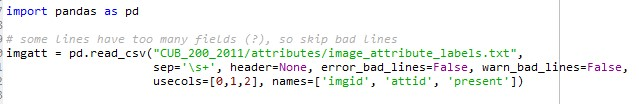
\includegraphics[scale=0.5]{figures/l2.jpg}
	\caption{Penyelesaian}
	\label{contoh}
	\end{figure}
\par Sehingga didapat hasil seperti berikut :
	\begin{figure}[!hbtp]
	\centering
	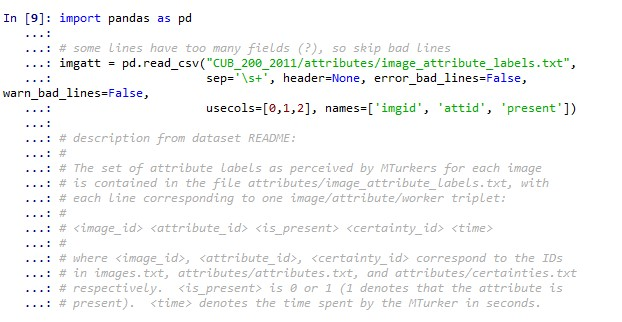
\includegraphics[scale=0.5]{figures/k41.jpg}
	\caption{Hasil}
	\label{contoh}
	\end{figure}
\end{enumerate}




\section{Rahmi Roza/1164085}
\subsection{Teori}
Penyelesaian Tugas Harian 5 ( No. 1-6 )
\begin{enumerate}
\item Random Forest Dan Ilustrasi Gambarnya
\begin{itemize}
\item Pengertian Random Forest:
\par Random Forest adalah suatu algoritma yang digunakan pada klasifikasi data dalam jumlah yang besar. Klasifikasi random forest dilakukan melalui penggabungan pohon  dengan melakukan training pada sampel data yang dimiliki. Penggunaan pohon (tree) yang semakin banyak akan mempengaruhi akurasi yang akan didapatkan menjadi lebih baik. Penentuan klasifikasi dengan random forest diambil berdasarkan hasil voting dari pohon yang terbentuk. Pemenang dari pohon yang terbentuk ditentukan dengan vote terbanyak. 
\par Pembangunan pohon  pada random forest sampai dengan mencapai ukuran maksimum dari pohon data. Akan tetapi,pembangunan pohon random foresttidak dilakukan pemangkasan  yang merupakan sebuah metode untuk mengurangi kompleksitas ruang.
\item Ilustrasi Gambar Random Forest :
\par

\begin{figure}[ht]
\centering
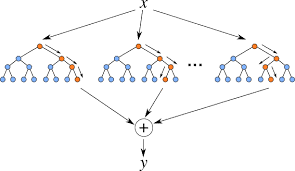
\includegraphics[scale=0.9]{figures/aku1.png}
\caption{Random Forest}
\label{contoh}
\end{figure}

\par
\end{itemize}

\item Cara Membaca Dataset, Dan artikan makna setiap file dan isinya.
\begin{itemize}
\item Cara Membaca Dataset :
\par (a) Buka Anaconda Navigator lalu jalankan Spyder, kemudian import libraries yang dibutuhkan.
\par (b) Masukkan kode python untuk membaca file csv, lalu jalankan.
\begin{figure}[ht]
\centering
\includegraphics[scale=0.5]{figures/21.jpeg}
\caption{(b)}
\label{contoh}
\end{figure}
\par (c) Maka pada window console akan menampilkan pesan berikut :
\begin{figure}[ht]
\centering
\includegraphics[scale=0.9]{figures/22.jpeg}
\caption{(c)}
\label{contoh}
\end{figure}
\par (d) Dari explorer dapat terlihat dataset yang terimport.
\begin{figure}[ht]
\centering
\includegraphics[scale=0.6]{figures/23.jpeg}
\caption{(d)}
\label{contoh}
\end{figure}
\par (e) Lalu klik dataset cell, maka akan muncul seperti berikut :
\begin{figure}[ht]
\centering
\includegraphics[scale=0.9]{figures/24.jpeg}
\caption{(e)}
\label{contoh}
\end{figure}
\par (f) Seperti yang terlihat pada gambar tersebut dataset ini memiliki Kolom Country, Age, dan Salary sebagai independent variable-nya dan kolom Purchased sebagai dependent variable-nya.
\par (g) Selanjutnya buat 2 matrix of features yang berisi values dari independent variable dan dependent variable.
\par (h) Lalu tuliskan perintah berikut :
\begin{figure}[ht]
\centering
\includegraphics[scale=0.9]{figures/25.jpeg}
\caption{(h)}
\label{contoh}
\end{figure}
\par (i) Perintah yang telah dibuat di atas akan membuat sebuah global environment baru dan muncul dataset.
\par (j) Klik dataset tersebut maka muncul tabel berisi dataset.

\end{itemize}

\item Cross Validation 
\begin{itemize}
\item Pengertian Cross Validation :
\par Cross Validation atau bisa disebut estimasi rotasi ,adalah sebuah teknik validasi model untuk menilai bagaimana hasil statistik analisis akan menggeneralisasi kumpulan data independen. Teknik ini utamanya digunakan untuk melakukan prediksi model dan memperkirakan seberapa akurat sebuah model prediktif ketika dijalankan dalam praktiknya. 
\par Dalam sebuah masalah prediksi, sebuah model biasanya diberikan kumpulan data (dataset) yang diketahui untuk digunakan dalam menjalankan pelatihan (dataset pelatihan), serta kumpulan data yang tidak diketahui (atau data yang pertama kali dilihat) terhadap model yang diuji (pengujian dataset).
\par Tujuan dari validasi silang adalah untuk mendefinisikan dataset untuk "menguji" model dalam tahap pelatihan (yaitu, validasi data), dalam rangka untuk membatasi masalah seperti terjadinya overfitting, memberikan wawasan tentang bagaimana model akan menggeneralisasi independen dataset (yaitu, tidak diketahui dataset, misalnya dari masalah nyata), dll.


\par
\end{itemize}
\item Penjelasan / Maksud Dari Score pada :
\begin{itemize}
\item Random forest ( 44\% )
\par Maksud arti score 44\%  pada random forest adalah hasil dari akurasi. Yang menggunakan 5 buah atribut yaitu dari 5 baris pertama dari set pelatihan yang akan memprediksi spesies 10, 28, 156, 10 dan 43.
\par

\item Decision Tree ( 27\% )
\par Maksud arti score 27\% pada decission tree adalah presentasi hasil dari perhitungan dataset. Dari set tentang burung pipit. Confusion matrix memberi tau hal-hal yang diharapkan, artinya, butrung-burung yang terlihat mirip saling bingung satu sama lain. 
\par

\item SVM ( 29\% )
\par Maksud arti score 29\% dari SVM adalah hasil pendekatan jaringan saraf. Di sini, akurasinya adalah 27\%, yang kurang dari akurasi 44\% sebelumnya. Oleh karena itu, dessicion tree menjadi  lebih buruk. Jika kita menggunakan Support Vector Machine (SVM), yang merupakan neural pendekatan jaringan, outputnya 29\%. Jadi 29\% pada SVM merupakan hasil otputannya.
\par
\par Hasil tersebut didapat dari hasil valdasi silang untuk memastikan bahwa membagi training test dengan cara yang berbeda. Sehingga didapat outputnya 44\% untuk hutan acak, 27\% untuk pohon keputusan, dan 29\% untuk SVM.
\par
\end{itemize}

\par
\item Confusion Matrix Dan Ilustrasinya
\begin{itemize}
\item Cara Membaca Confusion Matrix :
\par Perhitungan confusion matrix adalah sebagai berikut, akan saya beri contoh sederhana yaitu pengambilan keputusan untuk mendapatkan bantuan beasiswa. Saya menggunakan dua atribut, yaitu rekening listrik dan gaji. Yang pertama kita lakukan yaitu mencari 4 nilai yaitu a,b,c, dan d:
\par a= 4
\par b= 1
\par c= 1
\par d= 2
\par Kemudian kita dapat mencari nilai Recall, Precision, accuracy dan Error Rate
\par Recall =2/(1+2) = 0,66
\par  Precision = 2/(1+2) = 0,66
\par Accuracy =(4+2)/(4+1+1+2) = 0,75
\par Error Rate =(1+1)/(4+1+1+4) = 0,2
\par Ilustrasi Confusion Matrix :
\par
\begin{figure}[ht]
\centering
\includegraphics[scale=0.8]{figures/aku3.jpg}
\caption{Confussion Matrik}
\label{contoh}
\end{figure}
\end{itemize}

\par
\par
\item Voting Random Forest Dan Ilustrasi Gambarnya.
\par
\begin{itemize}
\item Pengertian Voting pada Random Forest	:
\par Metode ensemble dapat mencapai akurasi tinggi dengan membangun beberapa pengklasifikasi dan menjalankan
masing-masing secara mandiri. Ketika classifier membuat sebuah keputusan, kamu dapat memanfaatkan yang terbaik
keputusan umum dan rata-rata. Jika kita menggunakan metode yang paling umum, itu disebut voting.
\item Ilustrasi Gambar Voting Random Forest :
\begin{figure}[ht]
\centering
\includegraphics[scale=1]{figures/aku2.png}
\caption{Voting Random forest}
\label{contoh}
\end{figure}
\end{itemize}
\end{enumerate}

\subsection{Praktek}
Penyelesaian Tugas Harian 6 ( No. 1-8 )
\begin{enumerate}
\item Aplikasi Sederhana Pandas dan Penjelasan Code ( Perbaris )
\begin{itemize}
\item Pandas:
\par 
\par
\begin{itemize}
\item Penjelasan Code Baris 1 : Mengimport library pandas dari python dengan inisiasi pd.
\par
\item Penjelasan Code Baris 2 : Variabel s1 mendefinisikan data menggunakan pandas series.
\par
\item Penjelasan Code Baris 3 : Mencetak output
\par
\item Penjelasan Code Baris 4 : Menampilkan data s1
\par
\item Penjelasan Code Baris 5 : Mencetak output
\par
\item Penjelasan Code Baris 6 : Mengubah data karakter menjadi numerik
\par
\item Penjelasan Code Baris 7 : Mempilkan data s2
\par
\end{itemize}
\item Hasil:
\par
\par
\begin{figure}[ht]
\centering
\includegraphics[scale=0.8]{figures/pandas.jpg}
\caption{Pandas}
\label{contoh}
\end{figure}
\par

\par
\par
\item Aplikasi Sederhana Numpy dan Penjelasan Code ( Perbaris )
\begin{itemize}
\item Code Numpy:
\par 
\par
\begin{itemize}
\item Penjelasan Code Baris 1 : Import library numpy
\par
\item Penjelasan Code Baris 2 : Menmapilkan versi dari numpy.
\par
\item Penjelasan Code Baris 3 : Menampilkan konfigurasi dari numpy.
\par
\end{itemize}
\item Hasil:
\par
\par
\begin{figure}[ht]
\centering
\includegraphics[scale=0.8]{figures/numpyy.jpg}
\caption{Numpy}
\label{contoh}
\end{figure}
\par
\par

\par
\par
\item Aplikasi Sederhana Matplotlib dan Penjelasan Code ( Perbaris )
\begin{itemize}
\item Code Matplotlib:
\par 
\par
\begin{itemize}
\item Penjelasan Code Baris 1 : Mengimport library matplotlib dari python dengan inisiasi plt.
\par
\item Penjelasan Code Baris 2 : Variabel X
\par
\item Penjelasan Code Baris 3 : Variabel Y
\par
\item Penjelasan Code Baris 4 : Menampilkan nilai dari X
\par
\item Penjelasan Code Baris 5 : Menampilkan value dari X
\par
\item Penjelasan Code Baris 6 :  Menampilkan value dari variabel Y
\par
\item Penjelasan Code Baris 7 : Menampilkan nilai dari variabel Y
\par
\item Penjelasan Code Baris 8 : Mengatur label sumbu x dari sumbu saat ini.
\par
\item Penjelasan Code Baris 9 : Mengatur label sumbu y dari sumbu saat ini.
\par
\item Penjelasan Code Baris 10 : Menetapkan judul atau title.
\par
\item Penjelasan Code Baris 11 : Menampilkan figure atau gambar.
\par
\end{itemize}
\item Hasil:
\par
\par
\begin{figure}[ht]
\centering
\includegraphics[scale=0.8]{figures/matplotlib.jpg}
\caption{Matplotlib}
\label{contoh}
\end{figure}
\par
\end{itemize}

\par
\par
\item Program Aplikasi Random Forest dan Penjelasan Keluarannya :
\begin{itemize}
\item Code Random Forest 1 :
\par
\begin{figure}[ht]
\centering
\includegraphics[scale=0.7]{figures/cod1.jpg}
\caption{Gambar1}
\label{contoh}
\end{figure}
\par
\begin{itemize}
\item Penjelasan : Membaca dataset. Codingan di atas menghasilkan variabel baru yaitu imgatt. Terdapat 3 kolom dan 3677856 baris data.
\par 
\par
\end{itemize}
\item Code Random Forest 2 :
\par
\begin{figure}[ht]
\centering
\includegraphics[scale=0.7]{figures/cod2.jpg}
\caption{Gambar2}
\label{contoh}
\end{figure}
\par
\begin{itemize}
\item Penjelasan : Codingan di atas berfungsi untuk melihat sebagian data awal dari dataset. Hasilnya terdapat pada gambar di atas setelah di eksekusi.
\par
\par
\end{itemize}
\item Code Random Forest 3 :
\par
\begin{figure}[ht]
\centering
\includegraphics[scale=0.7]{figures/cod3.jpg}
\caption{Gambar3}
\label{contoh}
\end{figure}
\par
\begin{itemize}
\item Penjelasan : Codingan di atas merupakan tampilan untuk menampilkan hasil dari dataset yang telah di run atau di eksekusi. Dimana pada gambar di atas 3677856 merupakan baris dan 3 adalah kolom.
\par
\par
\end{itemize}
\item Code Random Forest 4 :
\par
\begin{figure}[ht]
\centering
\includegraphics[scale=0.7]{figures/cod4.jpg}
\caption{Gambar 4}
\label{contoh}
\end{figure}
\par
\begin{itemize}
\item Penjelasan : Pada gambar di atas menmapilkan hasil dari variabel imgatt2. Dimana index nya 'imgid', kolom berisi 'attid' dan values atau nilainya berisi 'present'.
\par
\par
\end{itemize}
\item Code Random Forest 5 :
\par
\begin{figure}[ht]
\centering
\includegraphics[scale=0.7]{figures/cod5.jpg}
\caption{Gambar 5}
\label{contoh}
\end{figure}
\par
\begin{itemize}
\item Penjelasan : Pada gambar di atas menmapilkan hasil dari variabel imgatt2.head. Dimana dataset nya ada 5 baris dan 312 kolom.
\par
\par
\end{itemize}
\item Code Random Forest 6 :
\par
\begin{figure}[ht]
\centering
\includegraphics[scale=0.7]{figures/cod6.jpg}
\caption{Gambar 6}
\label{contoh}
\end{figure}
\par
\begin{itemize}
\item Penjelasan : Pada gambar di atas menampilkan jumlah dari baris dan kolom dari variabel imgatt2. Dimana 11788 adalah baris dan 312 adalah kolom.
\par
\par
\end{itemize}
\item Code Random Forest 7 :
\par
\begin{figure}[ht]
\centering
\includegraphics[scale=0.7]{figures/cod7.jpeg}
\caption{Gambar 7}
\label{contoh}
\end{figure}
\par
\begin{itemize}
\item Penjelasan : Pada gambar di atas menunjukkan load dari  jawabannya yang berisi " apakah burung tersebut ( subjek pada dataset ) termasuk dalam spesies yang mana ?. Kolom yang digunakan adalah imgid dan label, kemudian melakukan pivot yang mana imgid menjadi index yang artinya unik sehubungan dengan dataset yang telah dieksekusi.
\par
\par
\end{itemize}
\item Code Random Forest 8 :
\par
\begin{figure}[ht]
\centering
\includegraphics[scale=0.2]{figures/cod8.jpg}
\caption{Gambar 8}
\label{contoh}
\end{figure}
\par
\begin{itemize}
\item Penjelasan : Pada gambar di atas menunjukkan hasil dari variabel imglabels. Dimana menampilkan dataset dari imgid dan label. Dan dapat dilihat hasilnya dari gambar di atas.
\par
\par
\end{itemize}
\item Code Random Forest 9 :
\par
\begin{figure}[ht]
\centering
\includegraphics[scale=0.7]{figures/cod9.jpg}
\caption{Gambar 9}
\label{contoh}
\end{figure}
\par
\begin{itemize}
\item Penjelasan : Pada gambar di atas menunjukkan jumlah baris dan kolom dari variabel imglabels. Dimana hasil dari kodingan tersebut dapat dilihat setelah di run. 
\par
\par
\end{itemize}
\item Code Random Forest 10 :
\par
\begin{figure}[ht]
\centering
\includegraphics[scale=0.7]{figures/cod10.jpg}
\caption{Gambar 10}
\label{contoh}
\end{figure}
\par
\begin{itemize}
\item Penjelasan : Pada gambar diatas dikarenakan isinya sama, maka bisa melakukan join antara dua data yang diesekusi ( yaitu ada imgatt2 dan imglabels ), sehingga pada hasilnya akan didapatkan data ciri dan data jawaban atau labelnya sehingga bisa dikategorikan/dikelompokkan sebagai supervised learning. Jadi perintah untuk menggabungkan kedua data, kemudian dilakukan pemisahan antara data set untuk training dan test pada dataset yang dieksekusi.
\par
\par
\end{itemize}
\item Code Random Forest 11 :
\par
\begin{figure}[ht]
\centering
\includegraphics[scale=0.7]{figures/cod11.jpg}
\caption{Gambar 11}
\label{contoh}
\end{figure}
\par
\begin{itemize}
\item Penjelasan :Pada gambar di atas menghasilkan pemisahan dan pemilihan tabel ( memisahkan dan memilih tabel ). 
\par
\par
\end{itemize}
\item Code Random Forest 12 :
\par
\begin{figure}[ht]
\centering
\includegraphics[scale=0.7]{figures/cod12.jpg}
\caption{Gambar 12}
\label{contoh}
\end{figure}
\par
\begin{itemize}
\item Penjelasan : Pada gambar di atas menunjukkan hasil dari variabel dtatthead. Dimana data nya dapat dilihat pada gambar diatas. Dan dataset nya terdiri dari 5 baris dan 312 kolom.
\par
\par
\end{itemize}
\item Code Random Forest 13 :
\par
\begin{figure}[ht]
\centering
\includegraphics[scale=0.7]{figures/cod13.jpg}
\caption{Gambar 13}
\label{contoh}
\end{figure}
\par
\begin{itemize}
\item Penjelasan : Pada gambar di atas menunjukkan hasil dari variabel dflabel.head. Dimana berisikan data dari imgid dan label. Dan hasilnya dapat dilihat pada gambar di atas.
\par
\par
\end{itemize}
\item Code Random Forest 14 :
\par
\begin{figure}[ht]
\centering
\includegraphics[scale=0.7]{figures/cod14.jpg}
\caption{Gambar 14}
\label{contoh}
\end{figure}
\par
\begin{itemize}
\item Penjelasan : Pada gambar di atas merupakan pembagian dari data training dan dataset
\par
\par
\end{itemize}
\item Code Random Forest 15 :
\par
\begin{figure}[ht] 
\centering
\includegraphics[scale=0.7]{figures/cod15.jpg}
\caption{Gambar 15}
\label{contoh}
\end{figure}
\par
\begin{itemize} 
\item Penjelasan : Pada gambar di atas merupakan pemanggilan kelas RandomForestClassifier. max features yang diartikan berapa banyak kolom pada setiap tree.
\par
\par
\end{itemize}
\item Code Random Forest 16 :
\par
\begin{figure}[ht]
\centering
\includegraphics[scale=0.7]{figures/cod16.jpg}
\caption{Gambar 16}
\label{contoh}
\end{figure}
\par
\begin{itemize}
\item Penjelasan : Pada gambar di atas merupaka perintah untuk melakukan fit untuk membangun random forest yang sudah ditentukan dengan maksimum fitur sebanyak 50.
\par
\par
\end{itemize}
\item Code Random Forest 17 :
\par
\begin{figure}[ht]
\centering
\includegraphics[scale=0.7]{figures/cod18.jpg}
\caption{Gambar 17}
\label{contoh}
\end{figure}
\par
\begin{itemize}
\item Penjelasan : Pada gambar di atas menunjukkan hasil dari cetakan variabel dftrainatt.head.
\par
\par
\end{itemize}
\item Code Random Forest 18 :
\par
\begin{figure}[ht]
\centering
\includegraphics[scale=0.7]{figures/cod18.jpg}
\caption{Gambar 18}
\label{contoh}
\end{figure}
\par
\begin{itemize}
\item Penjelasan : Pada gambar di atas merupakan hasil dari variabel dftestatt da dftsetlabel. Dimana hasilnya dapat dilihat dari pada gambar di atas
\par
\par
\end{itemize}

\end{itemize}


\par
\par
\item Program Aplikasi Confusion Matrix dan Penjelasan Keluarannya :
\begin{itemize}
\item Code Confusion Matrix 1 :
\par
\begin{figure}[ht]
\centering
\includegraphics[scale=0.7]{figures/cod19.jpg}
\caption{Gambar 19}
\label{contoh}
\end{figure}
\par
\begin{itemize}
\item Penjelasan :  Pada gambar di atas merupakan kodingan untuk import confusiion matrik dari random forest. untuk hasilnya dapat dilihat dari gambar.
\par 
\par
\end{itemize}
\item Code Confusion Matrix 2 :
\par
\begin{figure}[ht]
\centering
\includegraphics[scale=0.7]{figures/cod20.jpg}
\caption{Gambar 20}
\label{contoh}
\end{figure}
\par
\begin{itemize}
\item Penjelasan : Pada gambar di atas merupakan tampilan dari variabel cm.
\par
\par
\end{itemize}
\item Code Confusion Matrix 3 :
\par
\begin{figure}[ht]
\centering
\includegraphics[scale=0.7]{figures/cod21.jpg}
\caption{Gambar 21}
\label{contoh}
\end{figure}
\par
\begin{itemize}
\item Penjelasan : Pada gambar di atas merupakan perintah untuk plot. Dan untuk hasilnya terpadat pada gambar di atas. 
\par
\par
\end{itemize}
\item Code Confusion Matrix 4 :
\par
\begin{figure}[ht]
\centering
\includegraphics[scale=0.7]{figures/cod22.jpg}
\caption{Gambar 22}
\label{contoh}
\end{figure}
\par
\begin{itemize}
\item Penjelasan : Pada gambar di atas merupakan kodingan untuk menyesuaikan sumbu dengan nama datanya makanya datset nya di lakukan dengan perintah di atas.
\par
\par
\par
\end{itemize}
\item Code Confusion Matrix 5 :
\par
\begin{figure}[ht]
\centering
\includegraphics[scale=0.7]{figures/cod23.jpeg}
\caption{Gambar 23}
\label{contoh}
\end{figure}
\par
\begin{itemize}
\item Penjelasan : Pada gambar di atas merupakan perintah plot dari gambar sebelumnya.
\par
\par
\par
\end{itemize}

\end{itemize}

\par
\par
\item Program Klasifikasi SVM dan Decision Tree Beserta Penjelasan Keluarannya :
\begin{itemize}
\item Code SVM :
\par
\begin{figure}[ht]
\centering
\includegraphics[scale=0.7]{figures/cod25.jpg}
\caption{SVM}
\label{contoh}
\end{figure}
\par
\begin{itemize}
\item Penjelasan : Pada gambar di atas cara untuk mencoba klasikasi dengan SVM dengan dataset yang sama.
\par 
\par
\end{itemize}
\item Code Decision Tree :
\par
\begin{figure}[ht]
\centering
\includegraphics[scale=0.7]{figures/cod24.jpg}
\caption{Decission Tree}
\label{contoh}
\end{figure}
\par
\begin{itemize}
\item Penjelasan : Pada gambar di atas merupakan cara untuk mencoba klasikasi dengan decission tree dengan dataset yang sama.
\par
\par
\end{itemize}
\end{itemize}



\par
\par
\item Program Cross Validation dan Penjelasan Keluarannya :
\begin{itemize}
\item Code Cross Validation 1 :
\par
\begin{figure}[ht]
\centering
\includegraphics[scale=0.7]{figures/cod26.jpg}
\caption{Cross Validation 1}
\label{contoh}
\end{figure}
\par
\begin{itemize}
\item Penjelasan : Pada gambar di atas merupakan Hasil dari cross validation random forest.
\par 
\par
\end{itemize}
\item Code Cross Validation 2  :
\par
\begin{figure}[ht]
\centering
\includegraphics[scale=0.7]{figures/cod27.jpg}
\caption{Cross Validation 2}
\label{contoh}
\end{figure}
\par
\begin{itemize}
\item Penjelasan : Pada gambar di atas merupakan hasil dari cross validation Decission tree.
\par
\par
\end{itemize}
\item Code Cross Validation 3 :
\par
\begin{figure}[ht]
\centering
\includegraphics[scale=0.7]{figures/cod28.jpg}
\caption{Cross Validation 3}
\label{contoh}
\end{figure}
\par
\begin{itemize}
\item Penjelasan : Pada gambar di atas merupakan hasil dari cross validation SVM.
\par
\par
\end{itemize}
\end{itemize}



\par
\par
\item Program Pengamatan Komponen Informasi dan Penjelasan Keluarannya :
\begin{itemize}
\item Code Pengamatan Komponen Informasi 1 :
\par
\begin{figure}[ht]
\centering
\includegraphics[scale=0.7]{figures/cod29.jpg}
\caption{Program Pengamatan Komponen Informasi 1}
\label{contoh}
\end{figure}
\par
\begin{itemize}
\item Penjelasan : Pada gambar di atas menunjukkan cara untuk mengetahui berapa banyak tree yang dibuat, berapa banyak atribut yang dipakai dan informasi lainnya menggunakan kode.
\par 
\par
\end{itemize}
\item Code Pengamatan Komponen Informasi 2 :
\par
\begin{figure}[ht]
\centering
\includegraphics[scale=0.7]{figures/cod30.jpg}
\caption{Program Pengamatan Komponen Informasi 2}
\label{contoh}
\end{figure}
\par
\begin{itemize}
\item Penjelasan : Pada gambar di atas merupakan cara untuk  melakukan plot informasi ini dengan kode di atas.
\par 
\par
\end{itemize}
\end{itemize}
\end{itemize}
\end{itemize}

\item Penanganan Error
\begin{itemize}
\item Skrinsut Error
\par
\begin{figure}[ht]
\centering
\includegraphics[scale=0.7]{figures/Error.jpg}
\caption{Error}
\label{contoh}
\end{figure}
\par
\begin{itemize}
\item Kode Error: file b'data/CUB 200 2011/attributes/image attributes labels.txt'
\par 
\item Solusi Pemecahan Error : Hapus Direktori data pada kode pastikan satu folder.
\par 
\par
\end{itemize}
\end{itemize}

\end{enumerate}



\section{Fadila/1164072}
\subsection{Teori}
Penyelesaian Tugas Harian 5 ( No. 1-6 )
\begin{enumerate}
\item Random Forest Dan Ilustrasi Gambarnya
\begin{itemize}
\item Pengertian Random Forest:
\par Random forest ( hutan acak ) atau biasa juga disebut dengan istilah random decision fores (hutan keputusan acak ) merupakan metode pembelajaran ensembel untuk klasifikasi, regresi yang beroperasi dengan membangun banyak pohon keputusan pada waktu pelatihan dan menghasilkan kelas yang merupakan mode kelas (klasifikasi) atau prediksi rata-rata (regresi) dari masing-masing pohon.
\item Ilustrasi Gambar Random Forest :
\par

\begin{figure}[ht]
\centering
\includegraphics[scale=0.2]{figures/random1.jpg}
\caption{random forest}
\label{contoh}
\end{figure}

\par
\end{itemize}
\item Cara Membaca Dataset, Dan artikan makna setiap file dan isinya.
\begin{itemize}
\item Cara Membaca Dataset :
\par Membaca Dataset
\begin{enumerate}
\item Langakh-langkah cara membaca dataset :
\begin{itemize}
\item Pertama-tama kita harus membuka Aplikasi yang digunakan untuk membuka datasetnya 
\item Yang saya gunakan ialah spyder dari Anaconda Navigator
\item Selanjutnya import libraries seperti numphy, pandas, matplotlib dll ( sesuai kebutuhan ).
\item Silahkan untuk memasukkan kode python yang digunakan untuk membaca file csv yang berada pada dataset 
\par dataset = pd.read\_.csv('Data.csv)
\par
\begin{figure}[ht]
\centering
\includegraphics[scale=0.6]{figures/data1.jpg}
\caption{random forest 1}
\label{contoh}
\end{figure}
\par
\par
\item Kemudian jalankan script python tersebut
\item Perhatikan pada bagian " window consolenya ", tampilan akan seperti berikut :
\par
\par
\begin{figure}[ht]
\centering
\includegraphics[scale=0.6]{figures/data2.jpg}
\caption{random forest 2}
\label{contoh}
\end{figure}
\par
\par
\item Dari window 'explorer' tersebut, kita dapat melihat dataset yang terimport.
\par Akan ada kolom nama, tipe, size dan values
\par
\begin{figure}[ht]
\centering
\includegraphics[scale=0.2]{figures/data3.jpg}
\caption{random forest 3}
\label{contoh}
\end{figure}
\par
\par
\item Lalu klik dataset cell, maka akan muncul seperti berikut :
\par
\par
\begin{figure}[ht]
\centering
\includegraphics[scale=0.4]{figures/data4.jpg}
\caption{random forest 4}
\label{contoh}
\end{figure}
\par
\par
\item Selanjutnya seperti yang dapat dilihat pada gambar tersebut untuk dataset ini memiliki Kolom Country, Age, dan Salary sebagai independent variablenya dan kolom Purchased sebagai dependent variablenya.
\item Kemudian pada code buatlah 2 matrix of features yang berisi values / nilai-nilai dari independent variable dan dependent variable yang sesuai.
\item Setelah semuanya selesai, maka silahkan tuliskan perintah berikut :
\par dataset = read.csv('Data.csv')
\par
\item Perintah/ script yang telah dibuat di atas akan membuat sebuah global environment 
\item Global environmentnya berupa environment baru dan muncullah dataset.
\item Silahkan untuk meng-Klik dataset tersebut, kemudian akan muncul tabel berisi dataset.
\end{itemize}
\end{enumerate}

\par
\end{itemize}
\item Cross Validation Dan Ilustrasi Gambar	:
\begin{itemize}
\item Pengertian Cross Validation :
\par Cross Validation (validasi silang) biasa disebut dengan estimasi rotasi, atau pengujian out-of-sample dimana merupakan salah satu dari berbagai teknik validasi model yang serupa untuk menilai bagaimana hasil analisis statistik akan digeneralisasikan ke set data independen. Hal ini (terutama) digunakan dalam pengaturan di mana tujuannya adalah prediksi, dan orang ingin memperkirakan seberapa akurat model prediksi akan dilakukan dalam praktek.
\par Untuk satu putaran validasi silang melibatkan mempartisi sampel data ke dalam himpunan bagian pelengkap, melakukan analisis pada satu subset (disebut set pelatihan), dan jugamemvalidasi analisis pada subset lainnya (disebut set validasi atau set pengujian).
\par

\begin{figure}[ht]
\centering
\includegraphics[scale=0.2]{figures/cross.jpg}
\caption{cross validation}
\label{contoh}
\end{figure}

\par Penjelasan : Pada contoh gambar, didefinisikan bahwa terjadi penilaian hasil analisis statistik yang telah berubah ke set data independen dan merupakan sebuah prediksi. Apabila prediksinya akurat maka tampilannya akan cross seperti gambar tersebut.
\par
\end{itemize}
\par
\item Penjelasan / Maksud Dari Score pada :
\begin{itemize}
\item Random forest ( 44 \% )
\par Maksudnya adalah akurasi. Dimana Hasil dari eksekusi variabel, parameter dll dari perhitungan code dan decision tree terkait akan diproses lagi untuk menghasilkan nilai akurasi. Dan untuk nilai akurasinya berupa 44 \%
\par
\item Decision Tree ( 27 \% )
\par Untuk score dari Decision Tree yang berupa 27 \% merupakan presentasi hasil dari perhitungan dataset yang telah dibaca dan diproses sebelumnya.
\par
\item SVM ( 29 \% )
\par Untuk nilai 29 \% dari SCV merupakan hasil pendekatan jaringan saraf. Jaringan saraf sendiri merupakan komponen jaringan utama dari sistem saraf. Sistem tersebut mengatur dan mengontrol fungsi tubuh dan aktivitas dan terdiri dari dua bagian:  (SSP) yang terdiri dari otak dan sumsum tulang belakang, dan percabangan saraf perifer dari sistem saraf tepi (SST) yang terdapat dalam pengolahan dataset terkait. 
\par

\par
\end{itemize}
\item Confusion Matrix Dan Ilustrasinya :
\begin{itemize}
\item Pengertian Confusion Matrix :
\par Pertama-tama confusion matrix ialah suatu metode yang digunakan untuk melakukan perhitungan akurasi pada konsep data mining.
\item Cara Membaca Confusion Matrix :
\par Untuk pembacaan dan pemahaman pada confusion matrix dapat memperhatikan penjelasan berikut
\begin{itemize}
\item Perhatikan : Apabila hasil prediksi negatif dan data sebenarnya merupakan negatif.
\item Perhatikan : Apabila hasil prediksi positif sedangkan nilai sebenarnya merupakan negatif.
\item Perhatikan : Apabila hasil prediksi negatif sedangkan nilai sebenarnya merupakan positif.
\item Perhatikan : Apabila hasil prediksi positif dan nilai sebenarnya merupakan positif.
\end{itemize}
\par
\par
\item Pembacaan Lanjutan ( lebih jelas ) Untuk Confusion Matrix :
\begin{enumerate}
\item Pastikan definisi dari 4 proses klasifikasi yang akan digunakan ada dalam confusion matrix.
\item 4 Istilah tersebut ada TP, TN, FP dan FN
\item Cara bacanya yaitu True Positive ( TP ), True Negative ( TN ), False Positive ( FP ) dan False Negative ( FN ).
\item Ada pendefinisian biner pada klasifikasi confusion matrix
\item Klasifikasi tersebut menghasilkan keluaran berupa 2 Kelas ( Positif dan Negatif ) dan penentuan TP, FP ( 1 klasifikasi positif ) , FN dan TN ( 1 klasifikasi negatif ).
\end{enumerate}
\par

\item Ilustrasi Gambar
\par

\begin{figure}[ht]
\centering
\includegraphics[scale=0.4]{figures/confusion.jpg}
\caption{confusion matrix}
\label{contoh}
\end{figure}

\par
\par Penjelasan : Pada gambar dapat dilihat bahwa cara membaca keluaran dari klasifikasi contoh tersebut dibaca 1 dan 0 ( yaitu iya atau tidak ). Untuk perhitungan lainnya pada klasifikasi untuk confusion marix memang bersifat mutlak atau hanya berada pada 2 pilihan.
\par
\par 
\end{itemize}

\par
\par
\item Voting Random Forest Dan Ilustrasi Gambarnya.
\par
\begin{itemize}
\item Pengertian Voting pada Random Forest	:
\par Voting merupakan metode yang paling umum digunakan dalam random forest. Ketika classifier membuat keputusan, Anda dapat memanfaatkan yang terbaik keputusan umum dan rata-rata yang didefinisikan ke dalam bentuk "voting".
\par Setelah pohon terbentuk,maka akan dilakukan voting pada setiap kelas dari data sampel. Kemudian, mengkombinasikan vote dari setiap kelas kemudian diambil vote yang paling banyak.Dengan menggunakan random forest pada klasifikasi data maka, akan menghasilkan vote yang paling baik.
\item Ilustrasi Gambar Voting Random Forest :
\begin{figure}[ht]
\centering
\includegraphics[scale=0.3]{figures/voting.jpg}
\caption{voting random forest}
\label{contoh}
\end{figure}
\par 
\par Penjelasan : Pada gambar terlihat bahwa terdapat mayoritas voting dimana datanya berasal dari pengolahan decision tree 1, 2 dan 3 . Ketiga decision tree tersebut telah dikelompokkan kedalam class yang berbeda. Selanjutnya setelah dikelompokkan kedalam voting maka akan dieksekusi lagi sehingga menghasilkan class akhir untuk random forest dari decision tree tersebut. 
\par
\end{itemize}
\par

\end{enumerate}


\subsection{Praktek}
Penyelesaian Tugas Harian 6 ( No. 1-8 )
\begin{enumerate}
\item Aplikasi Sederhana Pandas dan Penjelasan Code ( Perbaris )
\begin{itemize}
\item Code Pandas:
\begin{lstlisting}
import pandas as fadila
np_array = np.array([10, 20, 30, 40, 50])
print("NumPy array:")
print(np_array)
new_series = fadila.Series(np_array)
print("Converted Pandas series dari Fadila:")
print(new_series)
\end{lstlisting}
\par 
\par
\begin{itemize}
\item Penjelasan Code Baris 1 : 
\par Mengimport library / module pandas sebagai fadila
\item Penjelasan Code Baris 2 :
\par variabel np\_array mendefinisikan variabel np.array dimana terdapat beberapa parameter yang akan dieksekusi pada variabel tersebut
\item Penjelasan Code Baris 3 :
\par Mendefinisiikan perintah print dengan tulisan " Numpy array "
\item Penjelasan Code Baris 4 :
\par Melakukan perintah print / pencetakan untuk variabel np\_array
\item Penjelasan Code Baris 5 :
\par Mendefinisikan variabel baru yaitu new\_series dimana mengeksekusi fadila.series dengan variabel parameternya ialah np\_array
\item Penjelasan Code Baris 6 :
\par Mendefinisikan perintah print dengan tulisan " Converted pandas series dari fadila "
\item Penjelasan Code Baris 7 :
\par Melakukan perintah print / pencetakan terhadap variabel new\_series
\end{itemize}
\item Hasil Eksekusi :
\par
\par
\begin{figure}[ht]
\centering
\includegraphics[scale=0.4]{figures/pandasfadila.jpg}
\caption{pandas}
\label{contoh}
\end{figure}
\par
\end{itemize}


\par
\par
\item Aplikasi Sederhana Numpy dan Penjelasan Code ( Perbaris )
\begin{itemize}
\item Code Numpy:
\begin{lstlisting}
import numpy as fadila
x = fadila.ones((3,3))
print("Array Original:")
print(x)
print("0 berada di border sedangkan 1 berada dalam array")
x = fadila.pad(x, pad_width=1, mode='constant', constant_values=0)
print(x)
\end{lstlisting}
\par
\begin{itemize}
\item Penjelasan Code Baris 1 :
\par Mengimport library / module numpy sebagai fadila
\item Penjelasan Code Baris 2 :
\par Mendefinisikan variabel x dengan mengeksekusi fadila.ones dengan 2 parameter yaitu ( 3,3 )
\item Penjelasan Code Baris 3 :
\par Mendefinisikan perintah print dengan parameter tulisan yaitu (" Array Original " )
\item Penjelasan Code Baris 4 :
\par Melakukan Perintah print variabel X
\item Penjelasan Code Baris 5 :
\par Mendefinisikan perintah print dengan parameter tulisan yaitu (" 0 berada di border sedangkan 1 berada dalam array ")
\item Penjelasan Code Baris 6 :
\par Variabel x mengeksekusi fadila.pad dengan 4 variabel parameter yaitu ( x, pad\_width=1 , mode='constant], constant\_values=0 )
\item Penjelasan Code Baris 7 :
\par  Melakukan perintah print / pencetakan variabel X
\end{itemize}
\item Hasil Eksekusi :
\par
\par
\begin{figure}[ht]
\centering
\includegraphics[scale=0.4]{figures/numpyfadila.jpg}
\caption{numpy}
\label{contoh}
\end{figure}
\par
\par
\end{itemize}

\par
\par
\item Aplikasi Sederhana Matplotlib dan Penjelasan Code ( Perbaris )
\begin{itemize}
\item Code Matplotlib:
\begin{lstlisting}
import matplotlib.pyplot as fadila
# line 1 points
x1 = [10,20,30]
y1 = [20,40,10]
# plotting the line 1 points 
fadila.plot(x1, y1, label = "line 1")
# line 2 points
x2 = [10,20,30]
y2 = [40,10,30]
# plotting the line 2 points 
fadila.plot(x2, y2, label = "line 2")
fadila.xlabel('x - axis')
# Set the y axis label of the current axis.
fadila.ylabel('y - axis')
# Set a title of the current axes.
fadila.title('Dua atau line lebih pada plot yang sama 
	 dengan suitable legends ')
# show a legend on the plot
fadila.legend()
# Display a figure.
fadila.show()
\end{lstlisting}
\par
\begin{itemize}
\item Penjelasan Code Baris 1 :
\par Mengimport library / module matplotlib.pyplot sebagai fadila
\item Penjelasan Code Baris 2 :
\par Mendefinisikan / membuat variabel x1  dengan pengeksekusian 3 parameter yaitu ( 10,20,30 )
\item Penjelasan Code Baris 3 :
\par Mendefinisikan / membuat  variabel y1  dengan pengeksekusian 3 parameter yaitu ( 10,20,30 )
\item Penjelasan Code Baris 4 :
\par Mendefinisikan perintah fadila.plot dengan 3 parameter ( x1,y1 , label = 'line 1")
\item Penjelasan Code Baris 5 :
\par Mendefinisikan variabel x1  dengan pengeksekusian 3 parameter yaitu ( 10,20,30 )
\item Penjelasan Code Baris 6 :
\par Mendefinisikan / membuat  variabel x2  dengan pengeksekusian 3 parameter yaitu ( 10,20,30 )
\item Penjelasan Code Baris 7 :
\par Mendefinisikan / membuat  variabel y2  dengan pengeksekusian 3 parameter yaitu ( 40,10,30 )
\item Penjelasan Code Baris 8 :
\par Mendefinisikan perintah fadila.plot dengan 3 parameter yaitu ( x2,y2 , label = 'line 2")
\item Penjelasan Code Baris 9 :
\par Mendefinisikan perintah fadila.xlabel dengan parameter ( x-axis )
\item Penjelasan Code Baris 10 :
\par Mendefinisikan perintah fadila.ylabel dengan parameter ( y-axis )
\item Penjelasan Code Baris 11 :
\par Mendefinisikan perintah fadila.title dengan parameter tulisan yaitu ( " dua atau line lebih pada plot yang sama dengan suitable legends " )
\item Penjelasan Code Baris 12 :
\par Mendefinisikan perintah fadila.legend tanpa parameter
\item Penjelasan Code Baris 13 :
\par Mendefinisikan perintah fadila.show untuk menampilkan hasil eksekusi dari variabel fadila
\end{itemize}
\item Hasil Eksekusi :
\par
\par
\begin{figure}[ht]
\centering
\includegraphics[scale=0.3]{figures/matplotlibfadila.jpg}
\caption{matplotlib}
\label{contoh}
\end{figure}
\par
\end{itemize}

\par
\par
\item Program Aplikasi Random Forest dan Penjelasan Keluarannya :
\begin{itemize}
\item Code Random Forest 1 :
\par
\begin{figure}[ht]
\centering
\includegraphics[scale=0.2]{figures/ran1.jpg}
\caption{random forest}
\label{contoh}
\end{figure}
\par
\begin{itemize}
\item Penjelasan : Codingan tersebut akan menghasilkan sebuah variabel baru yaitu "imgatt" ( yang telah dibuat sebelumnya ) dengan tipe dataframe dan berupa matrix 2 dimensi. Terdapat 3 kolom dan 3677856 baris data. Bisa di check isi datanya karena berupa data frame. Codingan tersebut "Membaca" dan "Menampilkan" data yang berasal dari file "image\_attribute\_labels.txt".
\par 
\par
\end{itemize}
\item Code Random Forest 2 :
\par
\begin{figure}[ht]
\centering
\includegraphics[scale=0.4]{figures/ran2.jpg}
\caption{random forest 2}
\label{contoh}
\end{figure}
\par
\begin{itemize}
\item Penjelasan : Hasil dari codingan tersebut berfungsi untuk melihat data awal dari data/dataset yang dibaca dan diproses. Lebih jelasnya hanya untuk melihat isi paling atas dari data dan ditampilkan di console saat codingan dieksekusi.
\par
\par
\end{itemize}
\item Code Random Forest 3 :
\par
\begin{figure}[ht]
\centering
\includegraphics[scale=0.4]{figures/ran3.jpg}
\caption{random forest 3}
\label{contoh}
\end{figure}
\par
\begin{itemize}
\item Penjelasan : Codingan diatas akan menghasilkan dan juga mena-
\par mpilkan dari jumlah data pada dataset yang telah dieksekusi. Jumlah data/ sizenya akan berupa baris dan kolom dari data yang ada.
\par
\par
\end{itemize}
\item Code Random Forest 4 :
\par
\begin{figure}[ht]
\centering
\includegraphics[scale=0.2]{figures/ran4.jpg}
\caption{random forest 4}
\label{contoh}
\end{figure}
\par
\begin{itemize}
\item Penjelasan : Codingan tersebut menghasilkan tampilan variabel baru yaitu "imgatt2" . Fungsinya yaitu juga untuk merubah atribut menjadi kolom dengan menggunakan pivot layaknya excel. Yang membedakan antara "imgatt2" dan "imgatt1" ialah, jumlah dari data yang ditampilkan berbeda.
\par
\par
\end{itemize}
\item Code Random Forest 5 :
\par
\par
\begin{itemize}
\item Penjelasan : Hasil dari codingan tersebut berfungsi untuk melihat data awal dari data/dataset yang dibaca dan diproses pada variabel"  imgatt2 ". Lebih jelasnya hanya untuk melihat isi paling atas dari data dan ditampilkan di console saat codingan dieksekusi.
\par
\par
\begin{figure}[ht]
\centering
\includegraphics[scale=0.3]{figures/ran5.jpg}
\caption{random forest 5}
\label{contoh}
\end{figure}
\end{itemize}
\item Code Random Forest 6 :
\par
\begin{figure}[ht]
\centering
\includegraphics[scale=0.4]{figures/ran6.jpg}
\caption{random forest 6}
\label{contoh}
\end{figure}
\par
\begin{itemize}
\item Penjelasan : Codingan diatas akan menghasilkan dan juga menam-
\par pilkan dari jumlah data pada dataset yang telah dieksekusi pada variabel " imgatt2 ". Jumlah data/ sizenya akan berupa baris dan kolom dari data yang ada.
\par
\par
\end{itemize}
\item Code Random Forest 7 :
\par
\begin{figure}[ht]
\centering
\includegraphics[scale=0.2]{figures/ran7.jpg}
\caption{random forest 7}
\label{contoh}
\end{figure}
\par
\begin{itemize}
\item Penjelasan : Hasil dari codingan diatas menampilkan atau menunjukkan load dari  jawabannya yang berisi " apakah burung tersebut ( subjek pada dataset ) termasuk dalam spesies yang mana ?. Kedua kolom yang digunakan adalah imgid dan label, kemudian melakukan pivot yang mana imgid menjadi index yang artinya unik sehubungan dengan dataset yang telah dieksekusi.
\par
\par
\end{itemize}
\item Code Random Forest 8 :
\par
\begin{figure}[ht]
\centering
\includegraphics[scale=0.4]{figures/ran8.jpg}
\caption{random forest 8}
\label{contoh}
\end{figure}
\par
\begin{itemize}
\item Penjelasan : Hasil dari codingan tersebut berfungsi untuk melihat data awal dari data/dataset yang dibaca dan diproses pada variabel"  imglabels ". Lebih jelasnya hanya untuk melihat isi paling atas dari data dan ditampilkan di console saat codingan dieksekusi.
\par
\par
\end{itemize}
\item Code Random Forest 9 :
\par
\begin{figure}[ht]
\centering
\includegraphics[scale=0.2]{figures/ran9.jpg}
\caption{random forest 9}
\label{contoh}
\end{figure}
\par
\begin{itemize}
\item Penjelasan : Codingan diatas akan menghasilkan dan juga menam-
\par pilkan dari jumlah data pada dataset yang telah dieksekusi pada variabel " imglabels ". Jumlah data/ sizenya akan berupa baris dan kolom dari data yang ada.
\par
\par
\end{itemize}
\item Code Random Forest 10 :
\par
\begin{figure}[ht]
\centering
\includegraphics[scale=0.2]{figures/ran10.jpg}
\caption{random forest 10}
\label{contoh}
\end{figure}
\par
\begin{itemize}
\item Penjelasan : Codingan diatas dikarenakan isinya sama, maka bisa melakukan join antara dua data yang diesekusi ( yaitu ada imgatt2 dan imglabels ), sehingga pada hasilnya akan didapatkan data ciri dan data jawaban atau labelnya sehingga bisa dikategorikan/dikelompokkan sebagai supervised learning. Jadi perintah untuk menggabungkan kedua data, kemudian dilakukan pemisahan antara data set untuk training dan test pada dataset yang dieksekusi.
\par
\par
\end{itemize}
\item Code Random Forest 11 :
\par
\begin{figure}[ht]
\centering
\includegraphics[scale=0.2]{figures/ran11.jpg}
\caption{random forest 11}
\label{contoh}
\end{figure}
\par
\begin{itemize}
\item Penjelasan : Codingan ini menghasilkan pemisahan dan pemilihan tabel ( memisahkan dan memilih tabel ). Pada codingan ini dilakukan kegiatan untuk drop label yang berada di depan kemudian menggunakan label yang berada pada posisi paling belakang yang selanjutnya melakukan join terhadap 2 variabel tersebut yang tela dieksekusi.
\par
\par
\end{itemize}
\item Code Random Forest 12 :
\par
\begin{figure}[ht]
\centering
\includegraphics[scale=0.2]{figures/ran12.jpg}
\caption{random forest 12}
\label{contoh}
\end{figure}
\par
\begin{itemize}
\item Penjelasan : Codingan ini menunjukkan hasil pengecekan dari isi variabel df.att bagian head ( tampilan awal ) dari dataset yang dieksekusi.
\par
\par
\end{itemize}
\item Code Random Forest 13 :
\par
\begin{figure}[ht]
\centering
\includegraphics[scale=0.2]{figures/ran13.jpg}
\caption{random forest 13}
\label{contoh}
\end{figure}
\par
\begin{itemize}
\item Penjelasan : Codingan ini menunjukkan hasil pengecekan dari isi variabel df.label bagian head ( tampilan awal ) dari dataset yang dieksekusi.
\par
\par
\end{itemize}
\item Code Random Forest 14 :
\par
\begin{figure}[ht]
\centering
\includegraphics[scale=0.2]{figures/ran14.jpg}
\caption{random forest 14}
\label{contoh}
\end{figure}
\par
\begin{itemize}
\item Penjelasan : Hasil codingannya menunjukkan pembagian untuk data training dan data testing pada dataset. Dilakukan pembagian data menjadi dua bagian dimana untuk row/baris data pertama sebanyak 8000 dijadikan sebagai data training , kemudian 8000 data sisanya sebagai data testing pada pengeksekusiannya.
\par
\par
\end{itemize}
\item Code Random Forest 15 :
\par
\begin{figure}[ht]
\centering
\includegraphics[scale=0.2]{figures/ran15.jpg}
\caption{random forest 15}
\label{contoh}
\end{figure}
\par
\begin{itemize}
\item Penjelasan : Hasil dari codingan tersebut yaitu instalasi kelas random forest. Dimana pada pemrosesannya, dilakukan pemanggilan kelas Random Forest Classifier ( Klasifikasi Random Forest ). Pada codingan terdapat max features yang diartikan sebagai berapa banyak kolom pada setiap tree yang dieksekusi pada dataset. 
\par
\par
\end{itemize}
\item Code Random Forest 16 :
\par
\begin{figure}[ht]
\centering
\includegraphics[scale=0.4]{figures/ran16.jpg}
\caption{random forest 16}
\label{contoh}
\end{figure}
\par
\begin{itemize}
\item Penjelasan : Codingan tersebut menunjukkan fitting random forest dengan dataset training. Dimana pengeksekusiannya dilakukan fit untuk membangun random forest yang sudah ditentukan dengan maksimum fitur sebanyak 50 untuk perpohonnya ( dari dataset yang dieksekusi ).
\par
\par
\end{itemize}
\item Code Random Forest 17 :
\par
\begin{figure}[ht]
\centering
\includegraphics[scale=0.2]{figures/ran17.jpg}
\caption{random forest 17}
\label{contoh}
\end{figure}
\par
\begin{itemize}
\item Penjelasan : Codingan tersebut menunjukkan hasil dari prediksi dataset yang dieksekusi. 
\par
\par
\end{itemize}
\item Code Random Forest 18 :
\par
\begin{figure}[ht]
\centering
\includegraphics[scale=0.2]{figures/ran18.jpg}
\caption{random forest 18}
\label{contoh}
\end{figure}
\par
\begin{itemize}
\item Penjelasan : Codingan tersebut menunjukkan score perolehan dari klasifikasi dataset yang dieksekusi. Terdapat hasil besaran akurasi dari code yang dieksekusi sesuai dengan data yang digunakan.
\par
\par
\end{itemize}
\end{itemize}




\par
\par
\item Program Aplikasi Confusion Matrix dan Penjelasan Keluarannya :
\begin{itemize}
\item Code Confusion Matrix 1 :
\par
\begin{figure}[ht]
\centering
\includegraphics[scale=0.2]{figures/Con1.jpg}
\caption{confusion matrix 1}
\label{contoh}
\end{figure}
\par
\begin{itemize}
\item Penjelasan : Codingan diatas menunjukkan proses dari pembuatan confusion matrix dimana dilakukan pemetaan dan pemetakan confusion matrix terhadap data yang dieksekusi.
\par 
\par
\end{itemize}
\item Code Confusion Matrix 2 :
\par
\begin{figure}[ht]
\centering
\includegraphics[scale=0.2]{figures/con2.jpg}
\caption{confusion matrix 2}
\label{contoh}
\end{figure}
\par
\begin{itemize}
\item Penjelasan : Codingan ini menunjukkan hasil dari pembuatan pemetakan data yang dilakukan sebelumnya ( Code confusion mtrix 1 ). Hasilnya berupa matrix yang didalamnya terdapat angka dari hasil eksekusi confusion matrix itu sendiri. Memunculkan array dan dtype dari hasil pembuatan confusion matrix.
\par
\par
\end{itemize}
\item Code Confusion Matrix 3 :
\par
\begin{figure}[ht]
\centering
\includegraphics[scale=0.2]{figures/con3.jpg}
\caption{confusion matrix 3}
\label{contoh}
\end{figure}
\par
\begin{itemize}
\item Penjelasan : Codingan diatas melakukan plotting confusion matrix dimana dieksekusi beberapa parameter yang disesuaikan dengan data yang dieksekusi. Code ini hanya melakukan proses plotting dan tidak menunjukkan hasil plotting confusion matrixnya.
\par
\par
\end{itemize}
\item Code Confusion Matrix 4 :
\par
\begin{figure}[ht]
\centering
\includegraphics[scale=0.2]{figures/con4.jpg}
\caption{confusion matrix 4}
\label{contoh}
\end{figure}
\par
\begin{itemize}
\item Penjelasan : Codingan tersebut menunjukkan hasil dari pembacaan file classes.txt yang dieksekusi. Dilakukan ploting terhadap sumbu sesuai dengan nama data dan dilakukan penyettingan ( set ) sehingga memberikan hasil seperti pada gambar.
\par
\par
\end{itemize}
\item Code Confusion Matrix 5 :
\par
\begin{figure}[ht]
\centering
\includegraphics[scale=0.2]{figures/con5.jpg}
\caption{confusion matrix 5}
\label{contoh}
\end{figure}
\par
\begin{itemize}
\item Penjelasan : Codingan ini menghasilkan plot dari hasil perubahan label. Dimana proses plot yang dilakukan akan merubah label dari classes / data yang dieksekusi.
\par
\par
\end{itemize}

\end{itemize}

\par
\par
\item Program Klasifikasi SVM dan Decision Tree Beserta Penjelasan Keluarannya :
\begin{itemize}
\item Code SVM :
\par
\begin{figure}[ht]
\centering
\includegraphics[scale=0.2]{figures/svm1.jpg}
\caption{svm}
\label{contoh}
\end{figure}
\par
\begin{itemize}
\item Penjelasan : Codingan ini menunjukkan klasifikasi dengan decision tree dengan dataset yang sama. Tentunya pada pemrosesannya decision tree digunakan dan menghasilkan output dari klasifikasi tersebut.
\par 
\par
\end{itemize}
\item Code Decision Tree :
\par
\begin{figure}[ht]
\centering
\includegraphics[scale=0.2]{figures/dec1.jpg}
\caption{decision tree}
\label{contoh}
\end{figure}
\par
\begin{itemize}
\item Penjelasan : Codingan ini menunjukkan klasifikasi dengan SVM dengan dataset yang sama. Tentunya pada pemrosesannya SVM digunakan dan menghasilkan output dari klasifikasi tersebut.
\par
\par
\end{itemize}
\end{itemize}



\par
\par
\item Program Cross Validation dan Penjelasan Keluarannya :
\begin{itemize}
\item Code Cross Validation 1 :
\par
\begin{figure}[ht]
\centering
\includegraphics[scale=0.2]{figures/cross1.jpg}
\caption{cross validation 1}
\label{contoh}
\end{figure}
\par
\begin{itemize}
\item Penjelasan : Codingan tersebut menunjukkan hasil dari Cross Validation Random Forest. Pada pemrosesannya dilakukan pengecekan terhadap Cross Validation untuk Random Forest sesuai dengan data yang dieksekusi.
\par 
\par
\end{itemize}
\item Code Cross Validation 2  :
\par
\begin{figure}[ht]
\centering
\includegraphics[scale=0.2]{figures/cross2.jpg}
\caption{cross validation 2}
\label{contoh}
\end{figure}
\par
\begin{itemize}
\item Penjelasan : Codingan tersebut menunjukkan hasil dari Cross Validation Decision Tree. Pada pemrosesannya dilakukan pengecekan terhadap Cross Validation untuk Decision Tree sesuai dengan data yang dieksekusi.
\par
\par
\end{itemize}
\item Code Cross Validation 3 :
\par
\begin{figure}[ht]
\centering
\includegraphics[scale=0.2]{figures/cross3.jpg}
\caption{cross validation 3}
\label{contoh}
\end{figure}
\par
\begin{itemize}
\item Penjelasan : Codingan tersebut menunjukkan hasil dari Cross Validation SVM. Pada pemrosesannya dilakukan pengecekan terhadap Cross Validation untuk SVM sesuai dengan data yang dieksekusi.
\par
\par
\end{itemize}
\end{itemize}





\par
\par
\item Program Pengamatan Komponen Informasi dan Penjelasan Keluarannya :
\begin{itemize}
\item Code Pengamatan Komponen Informasi 1 :
\par
\begin{figure}[ht]
\centering
\includegraphics[scale=0.2]{figures/pe1.jpg}
\caption{pengamatan komponen informasi 1}
\label{contoh}
\end{figure}
\par
\begin{itemize}
\item Penjelasan : Codingan ini memberikan hasil pengamatan konponen informasi dimana pada pengeksekusiannya dapat diketahui berapa banyak tree yang dibuat, berapa banyak atribut yang dipakai dan informasi lainnya terkait kode yang digunakan.
\par 
\par
\end{itemize}
\item Code Pengamatan Komponen Informasi 2  :
\par
\begin{figure}[ht]
\centering
\includegraphics[scale=0.2]{figures/pe2.jpg}
\caption{pengamatan komponen informasi 2}
\label{contoh}
\end{figure}
\par
\begin{itemize}
\item Penjelasan : Codingan ini menunjukkan plot dari komponen informasi agar bisa dibaca dimana pada pemrosesannya plotting dilakukan pada informasi dengan menggunakan kode.
\par
\par
\end{itemize}
\end{itemize}


\par
\par
\subsection{Penanganan Error}
Penyelesaian Tugas Harian 6 ( Penanganan Error )
\begin{enumerate}
\item Menyelesaikan dan Membahas Penanganan Error :
\begin{itemize}
\item Error 1 :
\par 
\par
\begin{itemize}
\item Penjelasan Error 1 :
\par Error tersebut disebabkan karena pada bagian codingan "directory" file yang akan dieksekusi atau dipanggil tidak ada.
\begin{lstlisting}
FileNotFoundError: File b'/data/CUB_200_2011/attributes/
			image\_attribute\_labels.txt' does not exist
\end{lstlisting}
\item Penyelesaian Error 1 :
\begin{enumerate}
\item Pertama-tama perhatikan file yang akan dieksekusi yaitu " image\_atribute\_labels.txt" 
\item Pastikan file tersebut berada satu tempat ( directory ) dengan file bird-identifier.py yang digunakan sebagai codingan untuk pengeksekusian file
\item Selanjutnya hapus codingan dan sesuai seperti contoh codingan berikut :
\begin{lstlisting}
imgatt = pd.read_csv(image_attribute_labels.txt)
\end{lstlisting}
\par
\item Maka tidak akan terjadi error lagi
\par
\end{enumerate}
\end{itemize}
\par
\par
\begin{figure}[ht]
\centering
\includegraphics[scale=0.2]{figures/errorfadila1.jpg}
\caption{error 1}
\label{contoh}
\end{figure}
\par
\par
\par
\item Penjelasan Error 2 :
\par Error tersebut disebabkan karena pada bagian codingan "directory" file yang akan dieksekusi atau dipanggil tidak ada.
\begin{lstlisting}
FileNotFoundError: File b'/data/CUB_200_2011/attributes/
			image\_class\_labels.txt' does not exist
\end{lstlisting}
\item Penyelesaian Error 2 :
\begin{enumerate}
\item Pertama-tama perhatikan file yang akan dieksekusi yaitu " image\_class\_labels.txt" 
\item Pastikan file tersebut berada satu tempat ( directory ) dengan file bird-identifier.py yang digunakan sebagai codingan untuk pengeksekusian file
\item Selanjutnya hapus codingan dan sesuai seperti contoh codingan berikut :
\begin{lstlisting}
imglabels = pd.read_csv(image_class_labels.txt)
\end{lstlisting}
\par
\item Maka tidak akan terjadi error lagi
\par
\end{enumerate}
\par
\par
\begin{figure}[ht]
\centering
\includegraphics[scale=0.2]{figures/errorfadila2.jpg}
\caption{error 2}
\label{contoh}
\end{figure}
\par
\par
\par
\item Penjelasan Error 3 :
\par Error tersebut disebabkan karena pada bagian codingan "directory" file yang akan dieksekusi atau dipanggil tidak ada.
\begin{lstlisting}
FileNotFoundError: File b'/data/CUB_200_2011/attributes/classes.txt' does not exist
\end{lstlisting}
\item Penyelesaian Error 3 :
\begin{enumerate}
\item Pertama-tama perhatikan file yang akan dieksekusi yaitu " classes.txt" 
\item Pastikan file tersebut berada satu tempat ( directory ) dengan file bird-identifier.py yang digunakan sebagai codingan untuk pengeksekusian file
\item Selanjutnya hapus codingan dan sesuai seperti contoh codingan berikut :
\begin{lstlisting}
birds = pd.read_csv(classes.txt)
\end{lstlisting}
\par
\item Maka tidak akan terjadi error lagi
\par
\end{enumerate}
\par
\par
\begin{figure}[ht]
\centering
\includegraphics[scale=0.2]{figures/errorfadila3.jpg}
\caption{error 3}
\label{contoh}
\end{figure}

\end{itemize}
\end{enumerate}
\end{enumerate}